\section{Theorie}
\label{sec:Theorie}

Ultraschall ist eine Schallwelle mit einem Frequenzbereich von $20\,$kHz bis $1\,$GHz und somit nicht mehr für den
Menschen hörbar.

Diese Wellen könne unter anderem mit einem piezo-elektrischen Kristall, meist Quarze, erzeugt werden. In einem elektrischen Wechselfeld werden
diese Kristalle zu Schwingungen angeregt und strahlen dabei Ultrachallwellen ab.

Mithilfe von Ultrachall kann die Geschwindigkeit von Strömungen berechnet werden. Die Frequenz der Ultraschallwele wird beim Auftreffen auf ein bewegtes Objekt
gemäß des Doppler-Effekts verschoben. Dieser Effekt beschreibt die vergrößerung der Frequenz einer Scahllquelle, falls sich diese einem Empfänger nähert, oder der
Empfänger sich der Quelle nähert. Dementsprechend verringert sich die Frequenz falls sich die Quelle von dem Empfänger entfernt, oder sich
der Empfänger von der Quelle entfernt.

\begin{align}
  &\text{Für bewegte Quelle:} \: &\nu = \frac{\nu_0}{1 \mp \frac{v_S}{c}} \\
  &\text{Für bewegten Empfänger:} \: &\nu = \nu_0 \left(1 \pm \frac{v_E}{c}  \right)
\end{align}

Mit der Geschwindigkeit des Senders $v_S$ und der Geschwindigkeit des Empfängers $v_E$ und der Schallgeschwindigkeit des jeweiligen Mediums $c$.

Für die Frequenzverschiebung $\Delta \nu$ bei dem Auftreffen des Ultrachalls auf die Strömung unter einem Winkel gilt:
\begin{align}
  \Delta \nu = 2\nu \frac{v_E}{c}\cos{\alpha}
\end{align}

In Abbildung 1 ist die Beziehung des Winkels $\alpha$ mit $v_E$ dargestellt.

\begin{figure}[H]
  \centering
  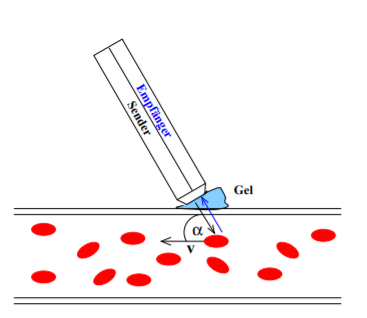
\includegraphics[height=5cm]{winkel.PNG}
  \caption{Verfahren zur Bestimmung des Geschwindigkeit von Strömungen. \cite{sample}}
  \label{fig:Linienspektrum}
\end{figure}
